\chapter{Experimentación}

\section{Análisis de la base de Datos}
    \noindent En esta sección se van a presentar el dataset con los datos para resolver el problema principal de este trabajo, así como el análisis previo a la manipulación de los mismos y el preprocesamiento realizado.

    \subsection{Base de datos proporcionada}
        \noindent El conjunto de datos Forense que se proporciona para resolver el problema presenta las siguientes características: 

        \begin{itemize}
            \item Contienen un total de \textbf{167 imágenes} de distintos sujetos. No se distribuye de forma equitativa el número de imágenes por sujeto, de manera que para algunos solo se dispone de una imagen mientras que otros disponen de varias. El sujeto con mayor número de imágenes tiene siete.
            \item La resolución de las imágenes también varía mucho, encontrando imágenes de alta calidad junto con otras con una muy baja resolución, oscilando entre los $4350 \times 3400$ píxeles y $168 \times 256$ píxeles.
            \item Hay imágenes a color y en escla de grises.
            \item Las imágenes se presentan en un conjunto muy variado de posiciones. Disponemos de: 
            \begin{itemize}
                \item $87$ imágenes frontales.
                \item $57$ imágenes con rostros en posición de $3/4$.
                \item $23$ imágenes de perfil.
            \end{itemize}
            \item Hay hasta un total de $30$ landmarks que pueden marcarse, aunque por regla general el número de landmarks en las imágenes es menor, como puede apreciarse en la \autoref{fig:Histograma}.
            \item En la \autoref{fig:Histograma} también podemos apreciar como la aparición de algunos landmarks es extremadamente baja, como es el caso del \textit{prosthion} y el \textit{Tragion} (tanto el izquierdo como el derecho). El resto de landmarks aparecen en más de la mitad de las imágenes. 
            \medskip
            \noindent La aparición en mayor o menor medida de cierto landmark en las imágenes nos sirve de indicador de si podrá ser o no aprendido por el modelo que usemos, de manera que los landmarks mencionados anteriormente, a causa del bajo número de ejemplos en los que aparecen puede ser más difícil que se aprendan.
        \end{itemize}

            \begin{figure}[!h]
                \centering
                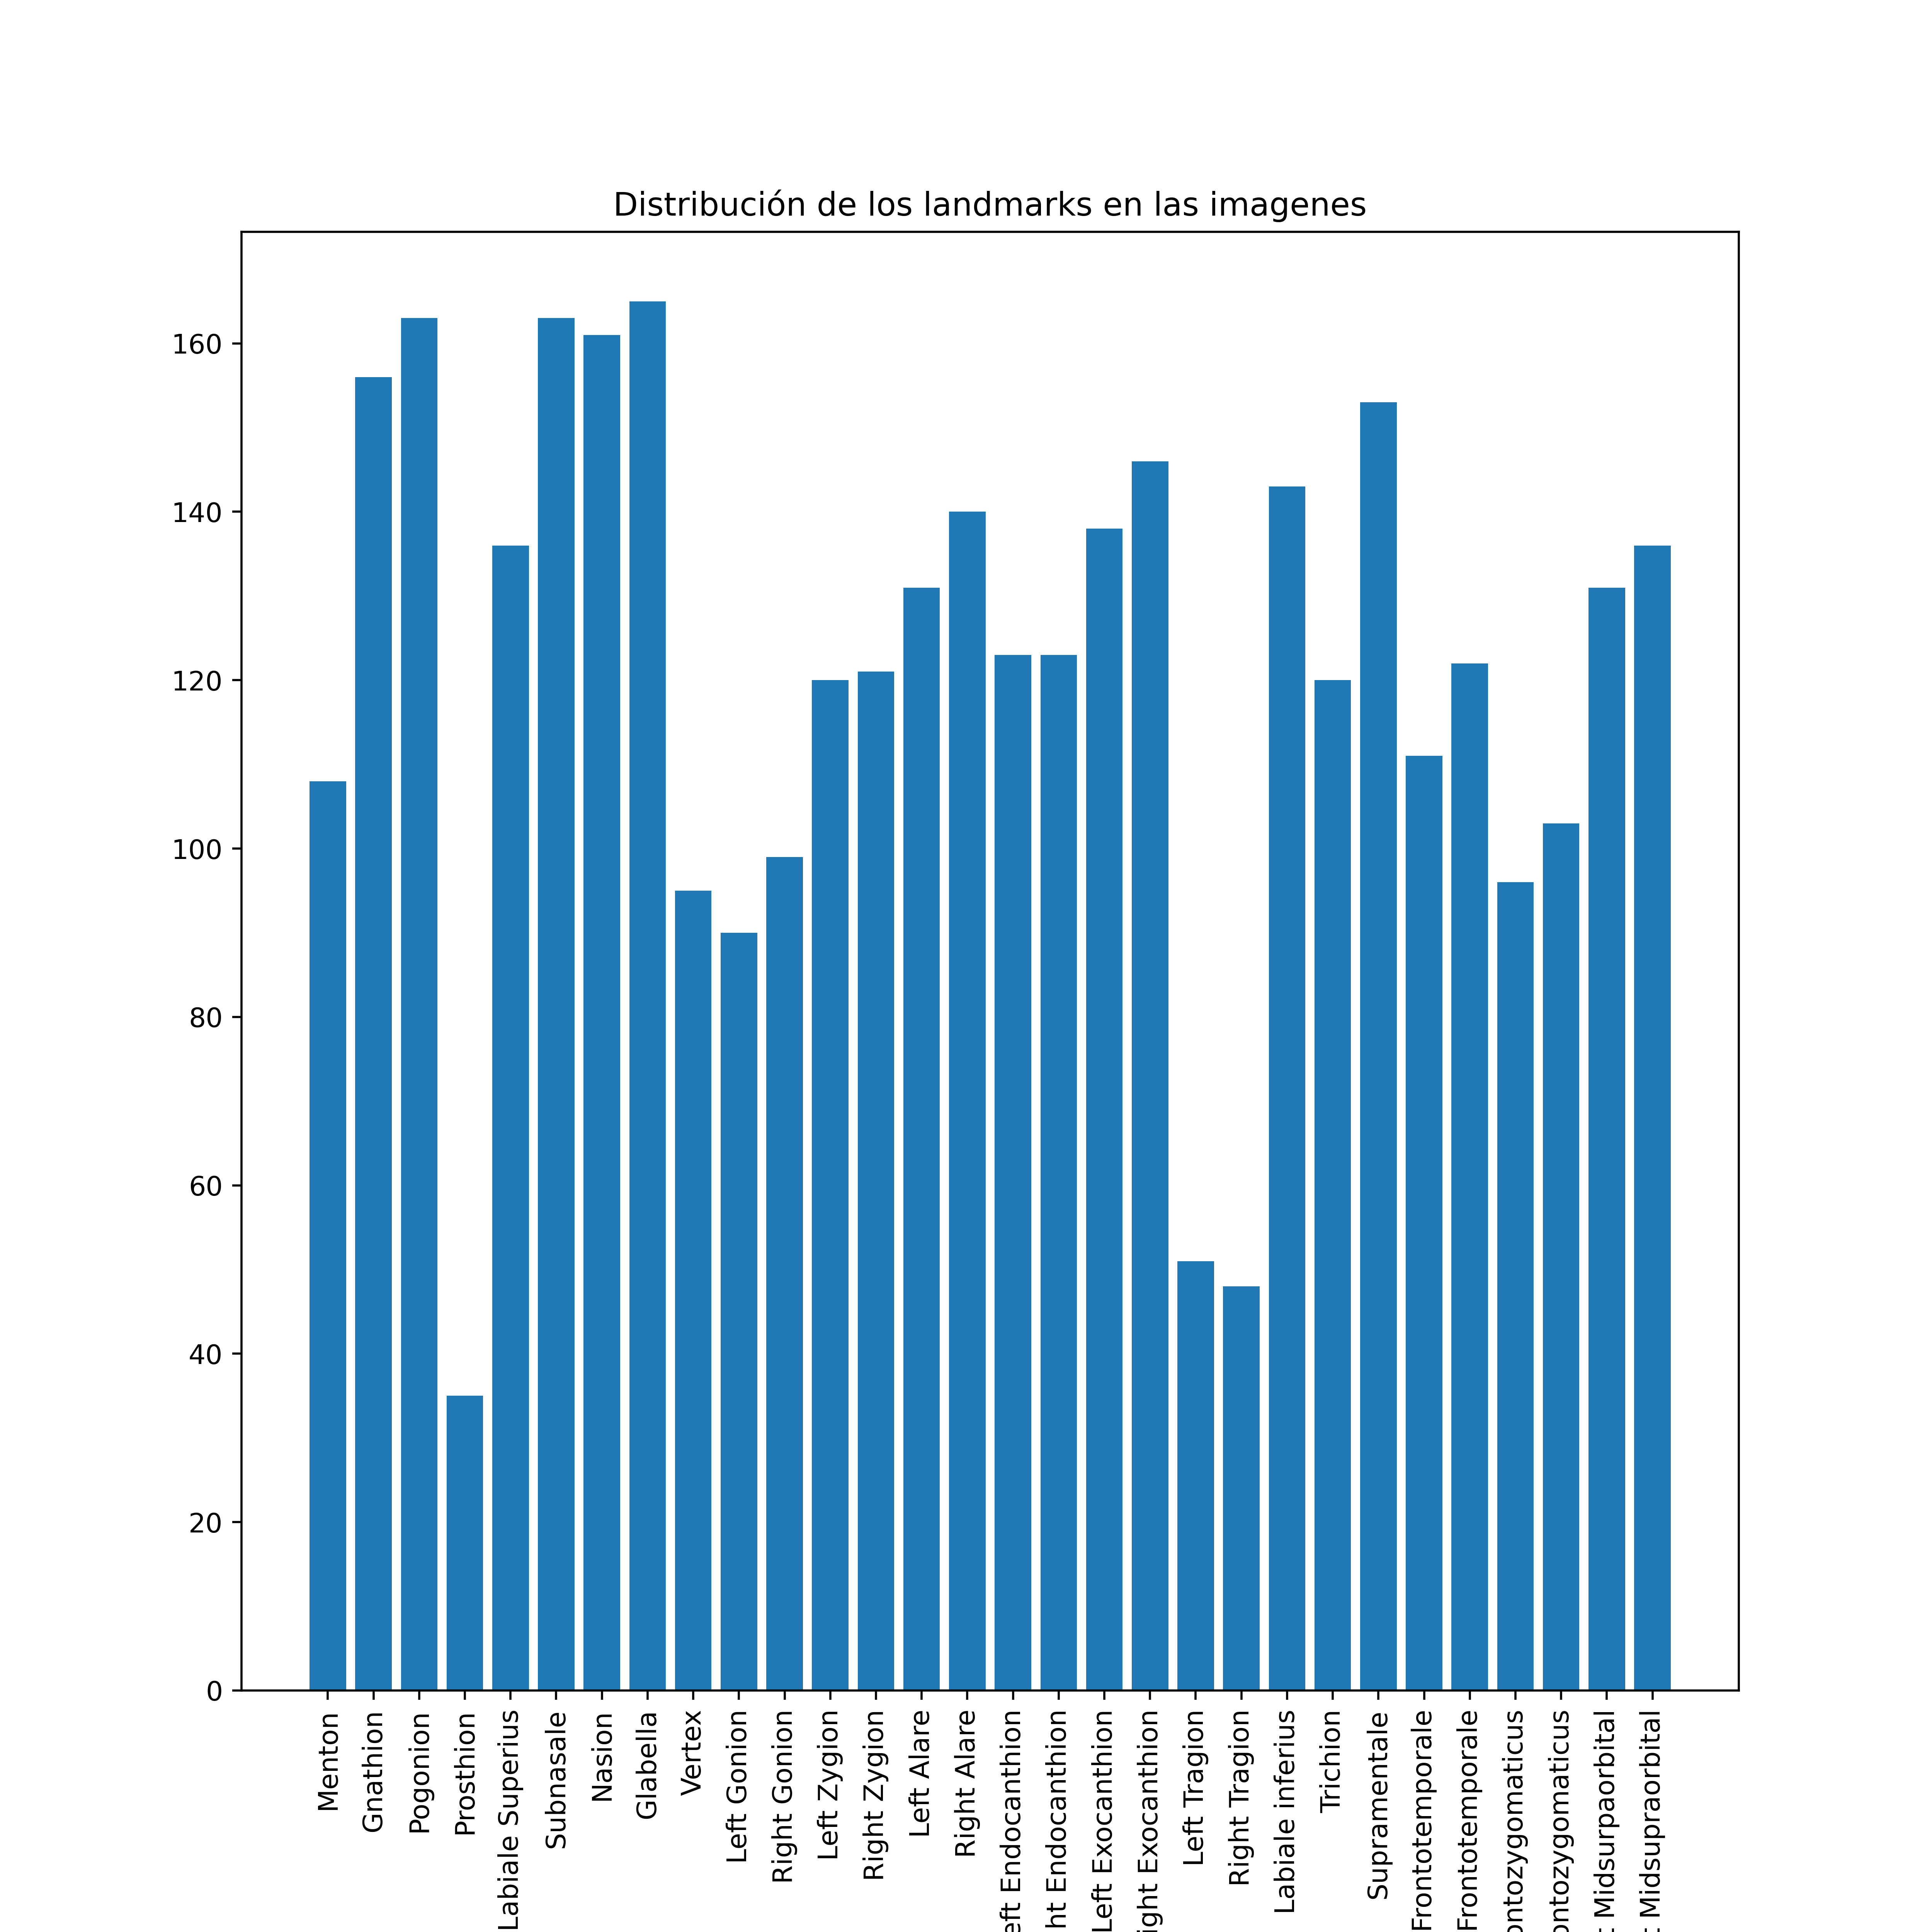
\includegraphics[width=0.9\textwidth]{img/distribucion_landmarks_imagenes.png}
                \caption{Histograma con la aparición de cada tipo de landmark en las imágenes del dataset.}
                \label{fig:Histograma}
            \end{figure}
    
    \subsection{Preprocesamiento}
        
        \subsubsection{Identificación de caras en las imágenes}
            \noindent Antes de poder entrenar el modelo, es necesario adecuar el dataset para que pueda usarse durante el entrenamiento. El framework está pensado para recibir como entrada una imagen a la cual se le hace un recorte a la región que ocupa el rostro con ayuda de un bounding box predefinido y determinado por las coordenadas en la imagen de las cuatro esquinas o bien siguiendo los landmarks descritos por el fichero auxiliar asociado a cada imagen. En nuestro caso, debido a que la mayoría de landmarks son internos y no se suelen situar en los bordes de la cara, hemos pensado que la mejor manera de entrenar la red es que serealice el recorte de la imagen de entrada de acuerdo a un \textit{bounding box}. Para ello fue necesario emplear una red especializada en la detección de caras en imágenes y que nos proporcionaba como salida una lista con los \textit{bounding boxes} de todas las caras detectadas, la red se denomina \textbf{Facenet} y que se puede importar de la librería \textit{facenet pytorch} como \textit{mtcnn}.

            \medskip

            \noindent Así pues, se realizó un primer estudio para determinar los mejores parámetros para \textit{facenet}. Existen muchos parámetros editables, pero la mayoría se dejaron con sus valores por defecto, únicamente se consideró modificar: 

            \begin{enumerate}
                \item \textbf{image size}: Determina el tamaño de la imagen de salida.
                \item \textbf{select largest}: Si su valor es \textit{true}, se devuelve la cara más grande detectada, y si su valor es \textit{false}, se devuelve la de mayor confianza detectada.
            \end{enumerate}


            \noindent En nuestro caso, primero se probó con un \textit{image size} de $256 \times 256$, pero esto tenía problemas pues en ocasiones no podían construirse bounding boxes de este tamaño y producían error, por lo que se redujo a $128 \times 128$ generando buenos resultados, por esto finalmente se dejó este valor. Por otro lado, observando las imágenes del dataset de entrenamiento, nos dimos cuenta que en algunas imágenes aparecían varios sujetos, y en ocasiones la cara más \entrecomillado{grande} mo pertenecía al sujeto principal. Es por ello que se decidió establecer el parámetro \textit{select largest} a \textit{False}, y así obtener como salida una lista de \textit{bounding boxes} ordenados de mayor a menor según el nivel de confianza.

            \medskip

            \noindent Una vez establecidos los parámetros, se detectaron problemas en la identificación de caras en algunas imágenes. Debido a que todas las imágenes erróneas estaban en escalas de grises nos dimos cuenta de que la red sólo acepta como entrada imágenes en tres canales, por lo que cada imagen en escala de grises de un solo canal tuvimos que replicar tres veces su canal. 
        
            \medskip
        
            \noindent Tras esto, volvimos a ver que en algunas imágenes no se detectaban \textit{bounding boxes}. Esto nos llevó a realizar un breve estudio sobre si era buena idea continuar usando esta red o buscar otra. En este estudio clasificamos las imágenes en tres grupos y aplicamos la red a cada uno de ellos por separado: 

            \begin{enumerate}
                \item Imágenes de sujetos en posición \textbf{ frontal}: en total hay $87$ imágenes frontales de las cuales se extraen correctamente el \textbf{$100\%$} de los \textit{bounding boxes}.
                \item Imágenes de sujetos en posición de \textbf{$3/4$}: En este caso hay $57$ imágenes de las cuales el \textbf{$100\%$} de los \textit{bounding boxes} extraidos por la red son correctos.
                \item Imágenes de sujetos en posición de \textbf{perfil}: En este caso hay un total de $23$ imágenes y se clasifican correctamente $20$, lo que supone una precisión del \textbf{$87\%$}. Además, las imágenes que fallaban estaban en escala de grises y con malas condiciones de calidad e iluminación.
            \end{enumerate}

            \noindent Por lo tanto, debido al bajo número de ejemplos en los que la red falla, se decidió mantener la red \textbf{Facenet} para determinar los \textit{bounding boxes} y además se excluyeron los tres ejemplos dónde fallaba del dataset, lo que hizo que en total se usaran $164$ de las $167$ imágenes originales.

            \medskip 

            \noindent Además, durante el estudio anterior se observaron otros hechos dignos de mención. En primer lugar se identificaron dos imágenes repetidas, pero se decidió mantenerlas pues los landmarks presentes en una y otra eran diferentes, lo que podía ayudar al entrenamiento. Por otro lado, durante el entrenamiento se vió cómo había una imagen de un determinado sujeto en la que aprecían simultáneamente dos fotos, una  de frente y otra de perfil, sin embargo, al estar los landmarks anotados únicamente en la imagen de frente se tomó el bounding box de la imagen frontal desechando el otro para el perfil. En otras dos imágenes se pueden ver un conjunto de varias personas, y la red mostraba erróneamente los \textit{bounding boxes} de personas que no eran el sujeto de estudio, por lo que estudiar cuál de todos los \textit{bounding boxes} devueltos pertenecía al sujeto correcto.

        \subsubsection{Creación del fichero annotations en el dataset}

            \noindent Una vez se identificaban correctamente todos los \textit{bounding boxes}, siguiendo como inspiración el dataset \textit{AFLW}, se generó un fichero denominado \textit{annotations.csv} dentro de la carpeta del proyecto en el que encuentra el dataset. En este fichero se almacenó \textbf{para cada imagen} una serie de datos: 

            \begin{itemize}
                \item El nombre del fichero.
                \item El índice de la imagen dentro del dataset. 
                \item Una lista con las coordenadas $2D$ de cada landmark en la imagen (incluidos los no presentes como situados en la posición $[-1,-1]$). 
                \item Una lista denominada máscara que representa la visibilidad de cada landmark en la imagen. Los landmarks visibles en la imagen tienen asociado el valor $1$, mientras que los no visibles tienen asociado el valor $0$.
                \item Finalmente, se almacena la posición de las cuatro esquinas que definen el \textit{bounding box}, para que el framework recorte la imagen quedándose con el rostro únicamente. 
            \end{itemize}

        \subsubsection{Reajuste de los bounding boxes}
            \noindent Finalmente, como parte del proceso de determinar los \textit{bounding boxes}, se vió que todos los casos, dichos rectángulos cortaban parte de las caras de los sujetos. En ocasiones partes en las que había landmarks marcados, es por ello, que se tuvo que realizar una transformación del \textit{bounding box} sugerido para que manteniendo el centro del mismo abarcase una mayor superficie y que contuviera el rostro completo del sujeto. 

            \medskip

            \noindent La transfomación consiste en desplazar la esquina superior izquierda del rectángulo una cantidad \textit{m} en el eje de ordenadas y abscisas y establecer el resto de esquinas de acuerdo a este parámetro como se muestra en la \autoref{fig:Transformacion_BB}.


            \begin{figure}[!h]
                \centering
                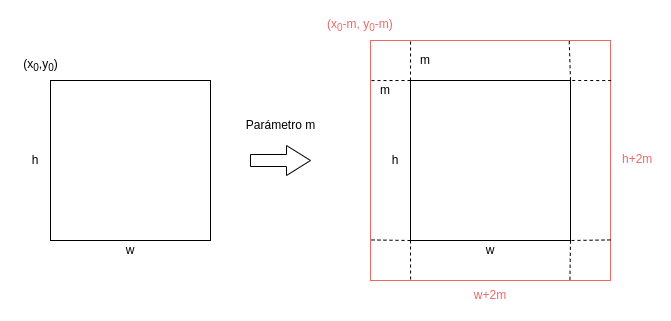
\includegraphics[width=0.8\textwidth]{img/Transformacion_rectangulo.png}
                \caption{Proceso seguido para la transformación.}
                \label{fig:Transformacion_BB}
            \end{figure}



    \subsection{Separación en conjuntos de entrenamiento y validación}
        \noindent En primer lugar separaremos el conjunto de datos que se proporciona en conjuntos de entrenamiento, validación y test. Debido a que trabajaremos con un conjunto de datos reducido será necesario emplear \textbf{validación cruzada} para la elección entre los modelos que se prueben. Así pues, de las \textbf{164 imágenes} que usaremos en total, establecemos una semilla para que los procesos aleatorios sean replicables en cualquier máquina y con ayuda de la función \textit{random-shuffle} de python separamos los datos en: 

        \begin{itemize}
            \item \textbf{Conjunto de test}: 33 imágenes ($20\%$ del total de imágenes).
            \item \textbf{Conjunto de entrenamiento:} 131 imágenes ($80\%$ del total de imágenes).
        \end{itemize}

        \noindent Por otro lado, el conjunto de entrenamiento se subdivide a su vez en cinco subconjuntos, con la idea de realizar \textbf{5-fold cross-validation}. Cada subconjunto estará compuesto por \textbf{26 imágenes} exceptuando el último que tendrá \textbf{27}.
        
        \medskip

        \noindent Para esta técnica se realizan cinco ejecuciones independientes en la cual se toman cuatro de los cinco subconjuntos de entrenamiento para entrenar el modelo y se deja el último subconjunto para validar el modelo. Con esta técnica, en cada iteración se cambia el conjunto que se empleará para validación, con la finalidad de mejorar la calidad de las decisiones que se tomen sobre el rendimiento, pues la decisión estará mejor informada. 

        \medskip

        \noindent De esta manera, con cada propuesta de modelo que realicemos, se medirá su rendimiento usando \textbf{5-fold cross-validation}, obteniendo 5 salidas de validación para cada modelo. La elección del mejor será mediante el cómputo de la mediana de estos para cada mdelo.

\section{Framework empleado}
               
    \subsection{Red empleada: 3FabRec}
        \noindent La red empleada para la resolución del problema es la desarrollada por \textbf{Bjorn Browatzki et al} en $2020$ \cite{browatzki20203fabrec} denominada \textbf{3FabRec}.La red en cuestión es un \textbf{Adversarial Autoencoder} combiando con una red \textit{GAN} (por la presencia de un segundo discriminante del estilo que hay en las GAN) que puede predecir landmarks gracias a la incorporación de unas capas convolucionales intermedias denominadas \textit{Interleaved Transfer Layer} en la etapa de reconstrucción y que explicaremos en profundidad más adelante.            

        \medskip

        \noindent Aplica un método \textit{semi-supervisado} en el cual:

        \begin{itemize}
            \item Hay una primera fase de \textbf{aprendizaje no supervisado} dónde se pretende adquirir conocimiento implícito sobre la estructura facial contenida en grandes conjuntos de imágenes de rostros de personas en diversas posiciones, iluminación y etnia. Para ello se codifica todo este conocimiento implícito en un vector de un espacio latente de baja dimensionalidad para posteriormente reconstruir la imagen. Este proceso se hace íntegramente en el \textit{Adversarial Autoencoder}.
            \item Posteriormente, en una segunda fase de \textbf{aprendizaje supervisado}, se entrena la red con un conjunto de imágenes etiquetadas con landmarks faciales que la red tratará de predecir. Para ello se intercalan entre las capas del generador capas de convolución encargadas de reconstruir los mapas de calor de cada landmark junto con la reconstrucción del rostro del paso previo.
            \item Finalmente, se puede incluir una tercera fase de \textit{finetuning} en la cual se entrena el Encoder para mejorar el rendimiento en la predicción de landmarks.
        \end{itemize} 

        \begin{figure}[!h]
            \centering
            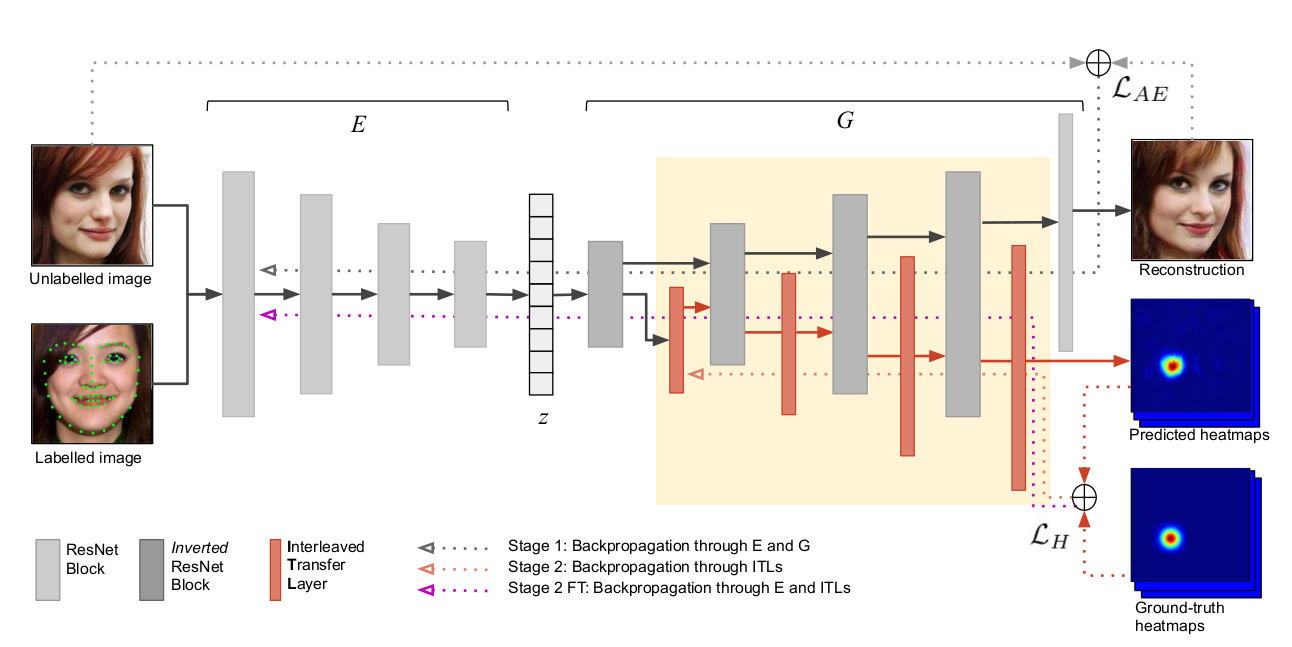
\includegraphics[width=0.7\textwidth]{img/3fabrec_arquitectura.png}
            \caption{Imagen resumen del framework 3FabRec. En ella podemos ver la estructura del \textit{Adversarial Autoencoder}, dividido en un Encoder (región bajo la \textit{E}) y un Generator (región bajo la \textit{G}) }
            \label{fig:3FabRec Resumen}
        \end{figure}

        \subsubsection{Arquitectura Adversarial Autoencoder}
            \noindent Para la construcción del \textit{Adversarial Autoencoder} emplean:
            
            \begin{itemize}
                \item \textbf{Encoder}: emplean una ResNet-$18$  hasta codificar la entrada en un vector de $99$ dimensiones. Está pensado para imágenes de res $256 \times 256 \times 3$, aunque se adapta también a imágenes de dimensiones $512 \times 512 \times 3$.
                \item \textbf{Decoder}: emplean la misma red ResNet-$18$ pero invertida.
            \end{itemize}

            \noindent Para una mejor comprensión he realizado unos diagramas con la herramienta \textit{diagrams.net}. En la \autoref{fig:bloque_encoder} podemos ver la estructura básica de los bloques de la ResNet-$18$.

            \begin{figure}[!h]
                \centering
                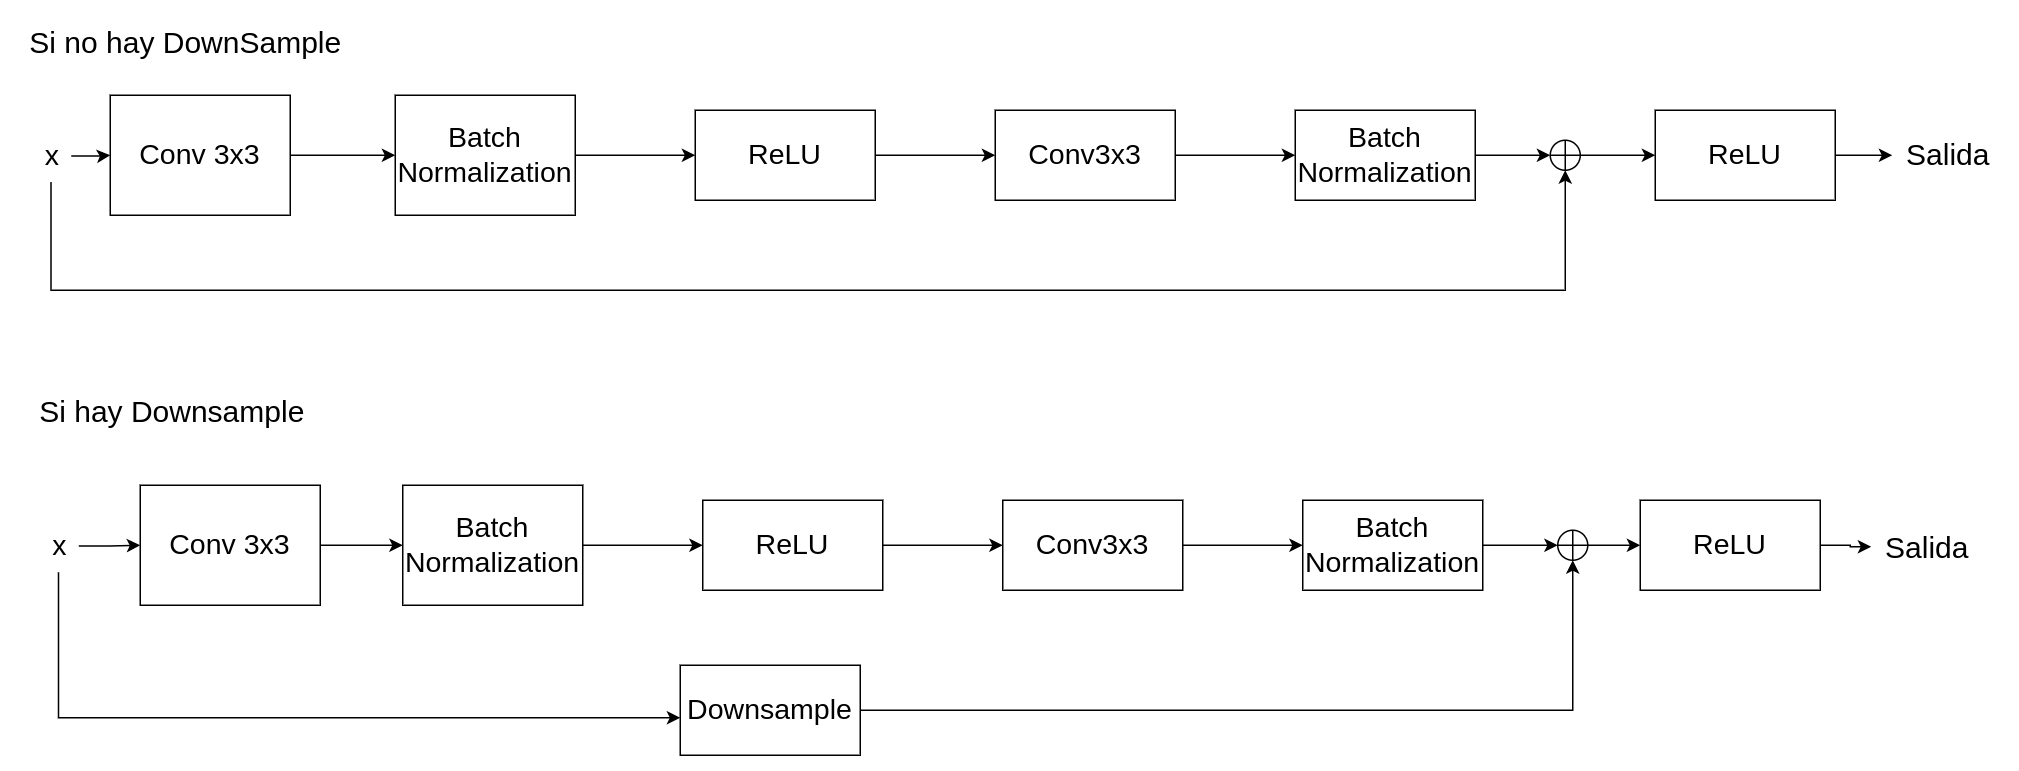
\includegraphics[width=0.7\textwidth]{img/bloque_basico_encoder.png}
                \caption{Bloques básicos que utilza la red ResNet-$18$ en sus capas. Se trata de una sucesión clásica de Convolución 3x3 + Batch Normalization + ReLU que se repite dos veces. En el primer caso los filtros de convolución no reducen las dimensiones del tensor añadiendo un padding de 1. En el segundo caso se reduce la dimensión del tensor a la mitad tras la primera convolución y se manteiene la dimensionalidad en la segunda. En el primer caso, la suma residual puede realizarse con el tensor x sin problema, en el segundo caso el tensor debe reducirse para que casen las dimensiones.}
                \label{fig:bloque_encoder}
            \end{figure}

            \medskip 

            \noindent Por otro lado en la \autoref{fig:Paso_encoder} podemos ver el paso de una imagen de entrada de tres canales y resolución $256 \times 256$ por el encoder.

            \begin{figure}[!h]
                \centering
                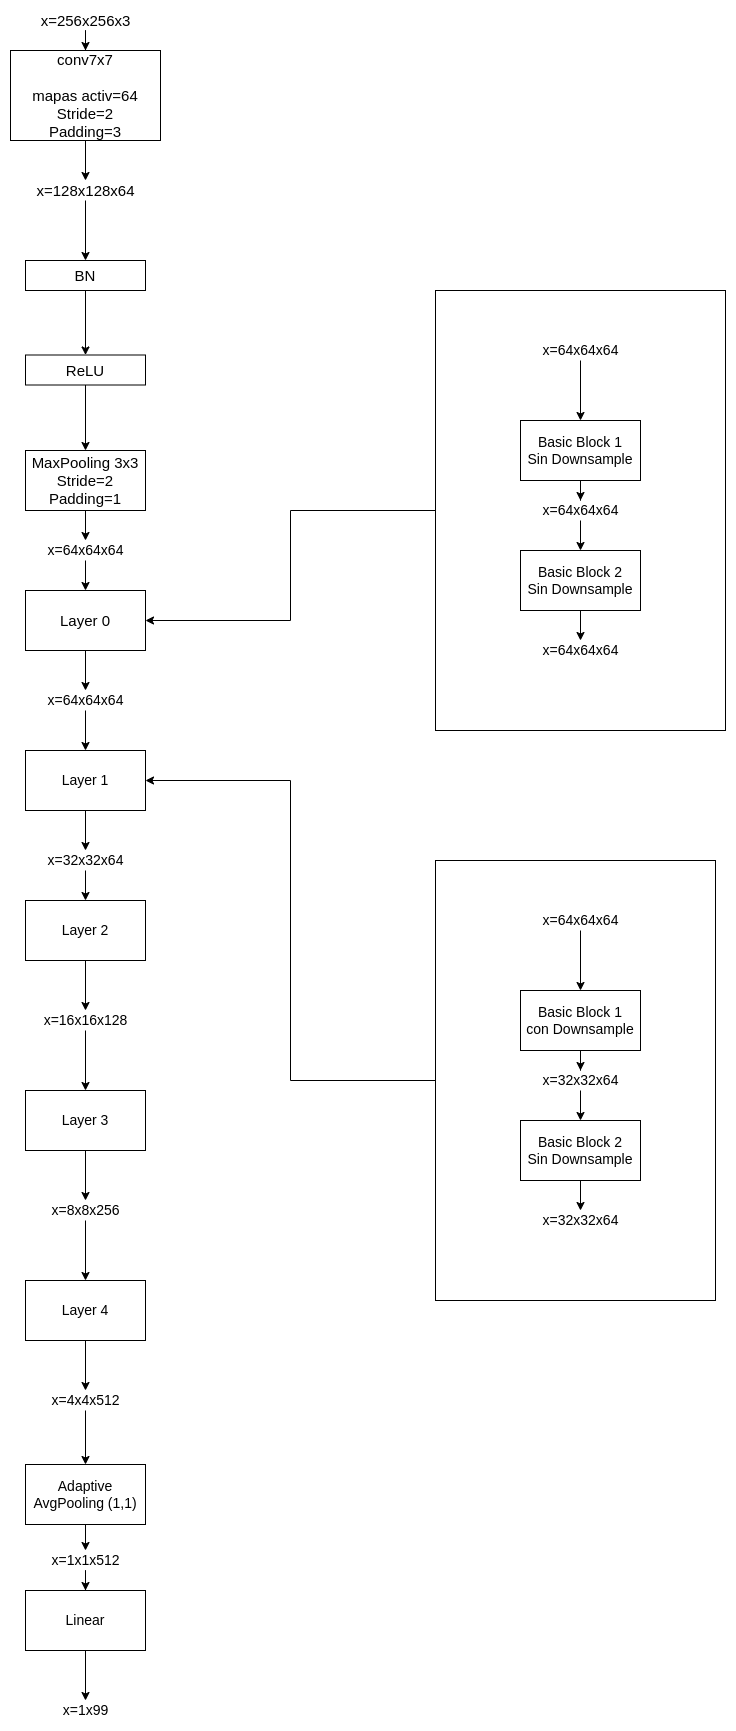
\includegraphics[width=0.7\textwidth]{img/3FabRec-Page-2.drawio.png}
                \caption{Ejemplo de paso de una imagen a través del Encoder. Cabe destacar que a partir de la Layer 1, todos los bloques tienen downsample.}
                \label{fig:Paso_encoder}
            \end{figure}

            \medskip

            \noindent En la \autoref{fig:Bloque_Decoder} podemos ver la estructura básica de un bloque en el Generador \textit{Inverse ResNet}, y un ejemplo del paso de un vector por el generador podemos verlo en la \autoref{fig:Paso_Generator}

            \begin{figure}[!h]
                \centering
                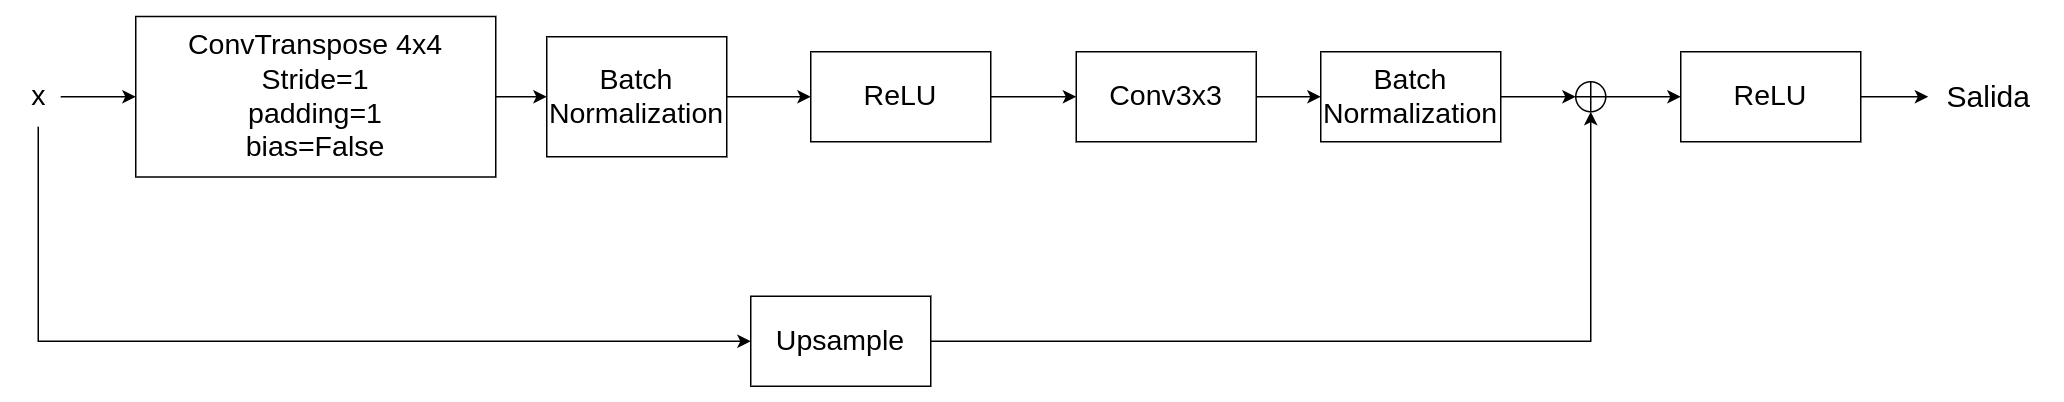
\includegraphics[width=0.7\textwidth]{img/bloque_invresnet.png}
                \caption{En primer lugar se aplica una convolución transpuesta que duplica las dimensiones del tensor de entrada y tras esto se sigue la misma estructura que en el bloque básico de la ResNet-$50$, la segunda convolución $3\times 3$ mantiene las dimensiones. Como consecuencia, para sumar el tensor de entrada con la salida del bloque se aumentan las dimensiones de este.}
                \label{fig:Bloque_Decoder}
            \end{figure}

            \begin{figure}[!h]
                \centering
                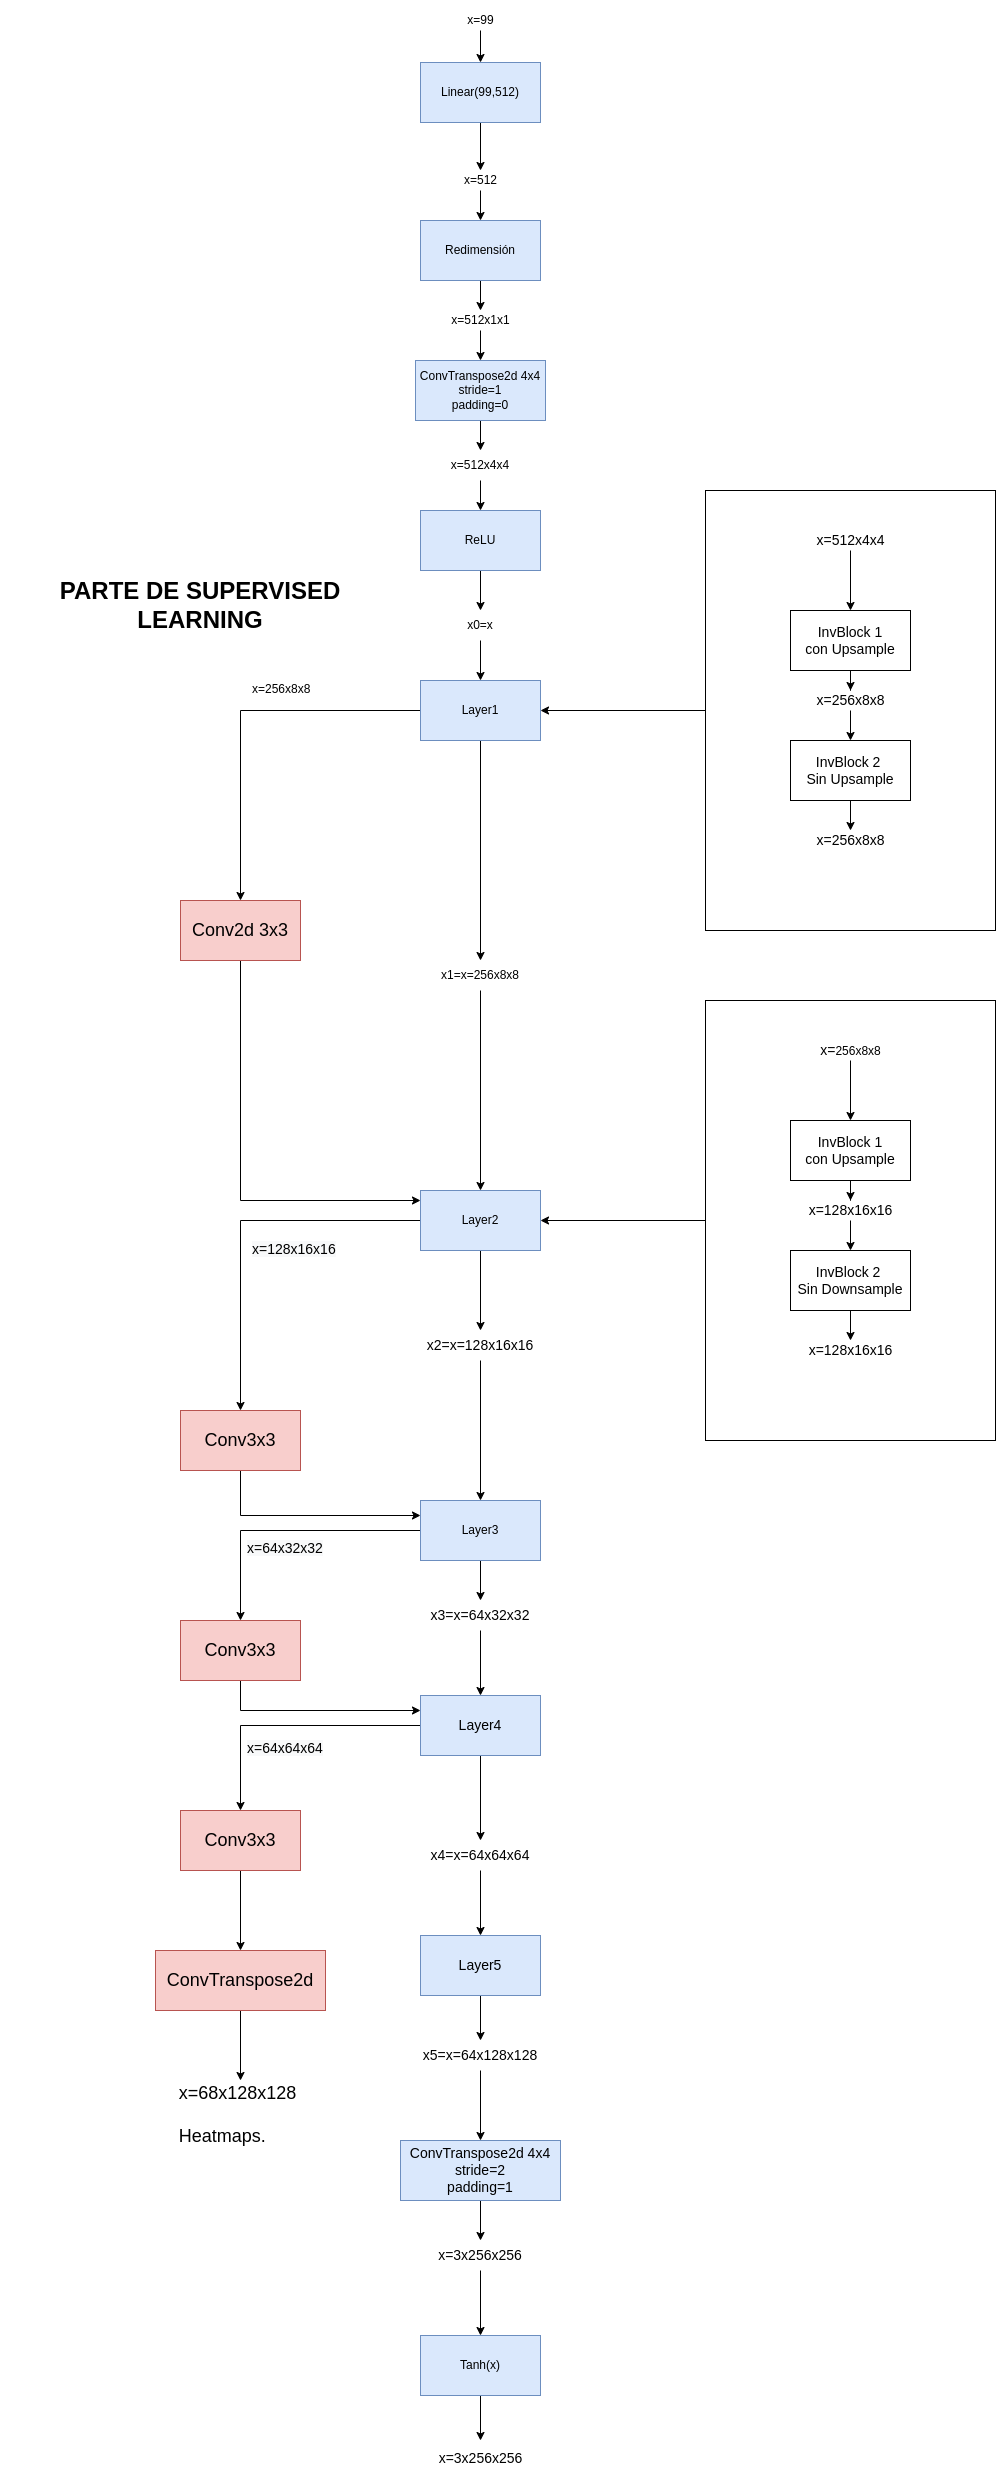
\includegraphics[width=0.5\textwidth]{img/paso_generator.png}
                \caption{Ejemplo del paso de un vector de $99$ dimensiones por el generador hasta reconstruirse la imagen de dimensiones $256 \times 256 \times 3$. La parte correspondiente al aprendizaje supervisado es la de los cuadrados azules, los cuadrados rojos corresponden a las \textit{ITLS} de la parte supervisada que se intercalan entre cada dos capas y dan como resultado los mapas de calor de los landmarks predichos.}
                \label{fig:Paso_Generator}
            \end{figure}

            \noindent Finalmente, para definir el autoencoder necesitamos un Discriminador, el cual que procure que los vectores del espacio vectorial latente sigan una determinada distribución. Dicha distribución será una normal multivariante estándar a la que vamos a añadirle un segundo discriminador propio de las redes \textbf{GAN} que nos dirá si la imagen reconstruida procede de la distribución que siguen los píxeles de la imagen de inicio. En la \autoref{fig:DGaussian} las redes neuronales que definen ambos discriminadores.

            \begin{figure}[!h]
                \centering
                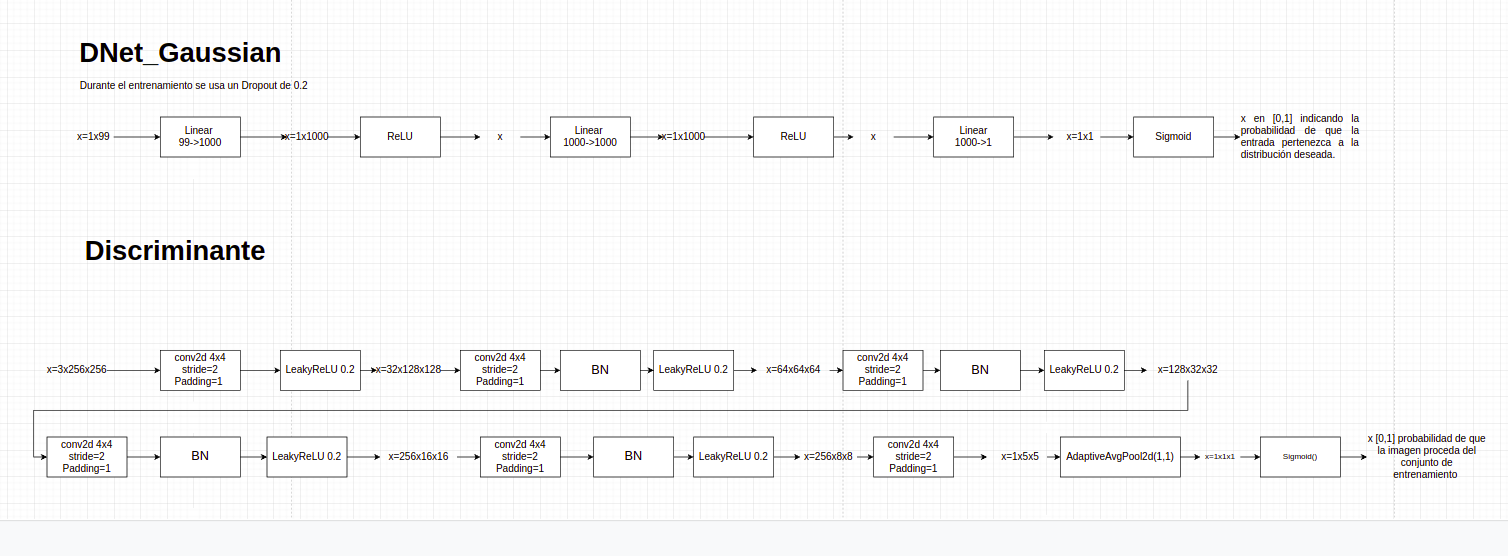
\includegraphics[width=0.99\textwidth]{img/DGaussian.png}
                \caption{En la imagen superior vemos el discriminante que se emplea para los vectores producidos por el Encoder y en la imagen inferior vemos el discriminante que se emplea para las imágenes generadas por el Generador. En ambos casos se da como salida un valor entre $0$ y $1$ que hace referencia a la probabilidad de pertenecer a la distribución deseada en el primer caso o a seguir la distribución de los píxeles de las imágenes en el segundo caso.}
                \label{fig:DGaussian}
            \end{figure}

        \subsubsection{Interleaved Transfer Layer (ITL)}
            
            \noindent Se tratan de simples capas convolucionales que se intercalan entre las capas del Generador. La última de estas capas proporciona como salida un conjunto de mapas de calor, uno por cada landmark predicho. Estos mapas de calor luego se emplean para representar en la imagen reconstruida los landmarks. La arquitectura de esta etapa podemos verla en la \autoref{fig:Paso_Generator}.
        
    \subsection{Función de pérdida}

        \noindent Para el entrenamiento de la red se emplean dos funciones de pérdida, la primera que presentaremos se emplea en el entrenamiento del \textit{Adversarial Autoencoder}, en la parte no supervisada, y la segunda función de pérdida se empleará tanto en la parte de aprendizaje supervisado como en la de \textit{finetuning} del Encoder.

        \medskip

        \noindent La función de pérdida empleada para el entrenamiento del \textit{Adversarial Autoencoder} en la parte de aprendizaje no supervisado es la siguiente: 
        
        \begin{align*}
            \min_{E,G} \max_{D_z,D_x} & \mathcal{L}_{AE}(E,G,D_z,D_x) = \\
            & \lambda_{rec} \mathcal{L}_{rec}(E,G) + \lambda_{cs}\mathcal{L}_{cs}(E,G) \\
            & + \lambda_{enc}\mathcal{L}_{enc}(E,D_z)+ \lambda_{adv} \mathcal{L}_{adv}(E,G,D_x)
        \end{align*}

        \noindent En la cual $\lambda_{enc}$ y $\lambda_{adv}$ toman el valor $1.0$ mientras que $\lambda_{rec}$ y $\lambda{cs}$ se establecen en $1.0$ y $60.0$ respectivamente. El valor de la función de coste se propagará por los pesos de $E$,$G$,$D_z$ y $D_x$ actualizándolos mediante \textit{back-propagation}.

        \medskip

        \noindent Por otro lado, la función de pérdida que se empleará en el entrenmiento de las \textit{ITLs} será la siguiente: 

        \begin{equation} \label{eq::L2}
            \mathcal{L}_H(ITL) = \mathbb{E}_{x ~ p(x)} \left[ \| H-ITL(a_1)\|_2 \right]
        \end{equation}

        \noindent Dónde $a_1$ serían los mapas de activación que genera el primer bloque de la ResNet invertida para la imagen codificada $z=E(x)$ (siendo $x$ la imagen de entrada a la red). En este caso se computa la distancia \textbf{$L_2$}entre los \textit{Heathmaps} de los lanmarks originales de la imagen $x$ de entrada, y los predichos por las \textit{ITLs}. Propagando el error por los pesos de las \textit{ITLS} solamente.

        \medskip

        \noindent A modo de aclaración, las imágenes etiquetadas con landmarks a la red suelen proporcionarse con el siguiente formato: 

        \begin{itemize}
            \item Un archivo con la imagen sin etiquetar. 
            \item Un archivo de texto plano con las coordenadas de cada landmark en la imagen.
        \end{itemize}

        \noindent Dados estos archivos, el framework, calcula para cada landmark proporcionado un mapa de calor en una imagen de tamaño $128 \times 128$ en el caso de que las imágenes de entrada sean de $256 \times 256$. Y es a ese conjunto de imágenes (una por cada landmark) a las que denominamos $H$ en la función anterior.

        \medskip

        \noindent Finalmente, en la etapa de \textit{fine-tuning} se computa la misma función de pérdida de antes, con la salvedad de que el error se propaga tanto por las \textit{ITLs} como por los pesos del \textit{Encoder}. Esto permite que el \textit{Encoder} se codifiquen con mayor precisión las imágenes y que se eliminen factores irrelevantes para la predicción de landmarks como son el género, el color de piel o la iluminación. Por otro lado se evita el overfitting ya que durante esta última etapa los pesos del \textit{Decoder} no se actualizan.

    \subsection{Proceso de entrenamiento de la red}

        \subsubsection*{Entrenamiento no-supervisado}
            \noindent El framework que empleamos ha sido entrenado durante $50$ épocas con imágenes de tamaño $256x256$ y con un tamaño de batch de $50$. En todas las etapas del entrenamiento se ha empleado un optimizador tipo Adam, el cual durante el entrenamiento del \textit{Adversarial Autoencoder} usó $\beta_1=0.0$ y $\beta_2=0.999$ con un \textit{learning rate} de $2\times 10^{-5}$.

            \medskip

            \noindent Por otra parte, se aplicaron técnicas de \textit{data-augmentation} a las imágenes de entrada como giros horizontales, traslaciones, \textit{resizing} o rotaciones.

        \subsubsection*{Entrenamiento supervisado}
            \noindent Para el entrenamiento de la parte supervisada, las imágenes de entrada se recortan de acuerdo a un \textit{bounding-box} creado por el framework a partir de unas coordenadas de entrada o bien de acuerdo a los landmarks que se proporcionan. Tras el recorte, se reescala la imagen hasta tener un tamaño de $256\times256$. 
            
            \medskip

            \noindent Por otro lado se crean los \textit{Heathmaps} para cada landmark. Para esto se crea una imagen de tamaño $128 \times 128$ por cada landmark marcando el punto con ayuda de una distribución normalde dos dimensiones centrada en las coordenadas del landmark y usando una desviación típica de $\sigma=7$.

            \medskip

            \noindent Tras esto se entrenan las cuatro \textit{ITLs}. A los datos de entrada se les aplican técnicas de \textit{data-augmentation} como rotaciones, traslaciones, reescalados y oclusiones. Para esta etapa se usa también un optimizador Adam con un \textit{learning rate} de $0.001$ y los mismos valores para $\beta_1$ y $\beta_2$.

            \medskip

            \noindent Finalmente, durante la etapa de \textit{fine-tuning} se establece un \textit{learning-rate} de $0.0001$ en las \textit{ITLs} mientras que el del \textit{Encoder} se mantiene en su valor por defecto de $2 \times 10^{-5}$ y cambiando el valor de $\beta_1 = 0.9$.

    \subsection{Bases de datos usadas por el framework}
        
        \noindent Para el entrenamiento no supervisado se emplearon los siguientes datasets unidos: 

        \begin{itemize}
            \item \textbf{VGGFace2} : Contiene un total de $3.3$ millones de imágenes de rostros en distintas poses, edad, iluminación, etnia, etc... Del dataset eliminaron las imágenes de rostros que tuviera una altura mayor a $100$ píxeles, quedando un total de $1.8$ millones de caras.
            \item \textbf{AffectNet} : Se trata de un dataset de $228$ mil imágenes en una gran variedad de poses, iluminación, etc..
        \end{itemize}

        \noindent En total usaron unas $2.1$ millones de imágenes.

        \noindent Para el entrenamiento no supervisado se emplearon los siguientes datasets: 

        \begin{itemize}
            \item \textbf{300-W} : une diversos datasets de rostros etiquetados con \textbf{$68$}landmarks de manera semi-automática como son \textbf{LFPW},\textbf{AFW}, \textbf{HELEN} y \textbf{XM2VTS}. Además de añadir datos propios. En total emplearon $3,148$ (aproximadamente el $80 \%$ )imágenes para el entrenamiento y $689$ para test, las cuales se dividieron en dos grupos, uno de $554$ imágenes considerado el grupo test estándar, y otro de $135$ imágenes difíciles.
            \item \textbf{AFLW} : contiene un total de $24,386$ imágenes \textit{in-the-wild} con un amplio rango de poses distintas. Se emplearon $20,000$ (aproximadamente el $80 \%$) imágenes para test y $4,386$ para entrenamiento. Las imágenes vienen etiquetadas con $21$ landmarks, pero en el framework se entrena la red para predecir \textbf{$19$}.
            \item \textbf{WFLW}: Es la más reciente de las empleadas y tiene un total de $10,000$ imágenes. Se usan $7,500$ para entrenamiento y $2,500$ para test. Las imágenes tienen un total de \textbf{$98$} landmarks anotados.
        \end{itemize}

\section{Experimentación}
    \subsection{Hipótesis iniciales}
        \noindent Debido a que partimos de \textbf{3fabRec}, un framework diseñado y probado de forma exahustiva por Björn Browatzki y Christian Wallraven, en Experimentación se va a respetar la arquitectura de la red en su totalidad, sin añadir ni eliminar capas. Del mismo modo debido a que la elección del optimizador \textbf{Adam} empleado por los autores ha sido fruto de un proceso de experimentación exahustiva por parte de los mismos no se va a probar a cambiarlo, además el optimizador Adam es adaptativo y tiene muy buen rendimiento en general, por lo que no tenemos ninguna razón que nos lleve a pensar que lograríamos grandes mejoras cambiando de optimizador.

        \medskip

        \noindent También, en la creación de los \textit{Heat maps} se ha optado por mantener el valor de $\sigma =7$ que se recomienda en el paper \cite{browatzki20203fabrec}, ya que de nuevo ha sido probado minuciosamente por los autores del framework.
    
    \subsection{Experimentación}
        \subsubsection{Modelo Base}
            \noindent En primer lugar se va a buscar un \textbf{modelo base} con el que obtener los primeros resultados y que iremos refinando hasta obtener el modelo solución. El framework \textbf{3FabRec} viene por defecto con cuatro modelos, todos ellos han sido entrenados en la fase de aprendizaje no supervisado, pero uno viene sin entrenamiento posterior de landmarks en ningún dataset, y los otros tres vienen con un entrenamiento en los datasets \textit{300w}, \textit{AFLW} y \textit{WFLW}. Así pues, la primera decisión a tomar es si emplear un modelo preentrenado en alguno de los datasets anteriores o utilizar uno sin entrenar. 

            \medskip

            \noindent Para tomar la anterior decisión se han repasado los diferentes datasets sobre los que se entrenó la red y se ha decidido que se usará como modelo base el que ha sido entrenado en \textit{AFLW}, debido a que el número de landmarks que predice este modelo es similar al de nuestro problema, ya que predice 21 landmarks, mientras que los demás modelos han sido entrenados para predecir 68 en el caso de \textit{300w} y 98 en el caso de \textit{WFLW}. Por otro lado, los landmarks que predice AFLW, pese a no tener una justificación biológica, son parecidos a los anotados en el dataset que se proporciona. Es por esto que consideramos una buena primera decisión emplear la red \textbf{preentrenada en AFLW}.

            %TODO INSERTAR IMAGEN DE LOS LANDMARKS DE AFLW vs LOS NUESTROS.

            \medskip

            \noindent Por otro lado, debido a que no conocemos todavía el efecto que tiene el entrenamiento con la etapa de \textit{fine-tuning} sobre los datos, vamos a realizar un entrenamiento únicamente de las \textbf{ITLs} durante un total de \textbf{40 épocas} hasta la convergencia del \textit{mse}, que es la medida de error entre los \textit{Heat maps} predichos por el modelo y los reales, y no utilizaremos técnicas de \textit{data augmentation}. Por otro lado, los parámetros que se han usado han sido los que sugieren por defecto en el framework, ya que aún no tenemos información suficiente sobre el rendimiento como para cambiarlos. Dichos valores son: 

            \begin{itemize}
                \item El \textit{learning rate} para el optimizador Adam usado en el entrenamiento de las ITLs se establece en $0.001$. 
                \item El valor del parámetro $\beta_1$ se establece en $0.0$.
                \item El valor del parámetro $\beta_2$ se establece en $0.9$.
            \end{itemize}

            \noindent Los resultados obtenidos por imagen en cada partición de \textbf{cross validation 5-fold } se pueden encontrar en \autoref{ap:apendiceA}. En estas tablas podemos observar la media del NME obtenido entre todos los landmarks presentes en la imagen, es decir, los no marcados no computan en esta media. Los resultados obtenidos son en general buenos, el NME no es muy elevado. Por otro lado vemos también el error de reconstrucción, que como podemos observar generalmente es elevado, lo que nos indica que no se están reconstruyendo fielmente las imágenes, algo que podría afectar al marcado de landmarks, puesto que estos se marcan en primer lugar sobre la imagen reconstruida, y luego se trasladan a la original.

            \begin{table}[!ht]
                \centering
                \caption{Media del error NME obtenido por landmark entre todas las particiones de cross-validation.}
                \begin{tabular}{|l|l|l|}
                \hline
                    ~ & Landmark & Media NME por landmark \\ \hline
                    0 & Menton & 3.944 \\ \hline
                    1 & Gnathion & 2.637 \\ \hline
                    2 & Pogonion & 2.549 \\ \hline
                    3 & Prosthion & 0.932 \\ \hline
                    4 & Labiale Superius & 2.099 \\ \hline
                    5 & Subnasale & 2.059 \\ \hline
                    6 & Nasion & 2.254 \\ \hline
                    7 & Glabella & 2.547 \\ \hline
                    8 & Vertex & 6.244 \\ \hline
                    9 & Left Gonion & 7.684 \\ \hline
                    10 & Right Gonion & 11.283 \\ \hline
                    11 & Left Zygion & 5.098 \\ \hline
                    12 & Right Zygion & 6.309 \\ \hline
                    13 & Left Alare & 1.939 \\ \hline
                    14 & Right Alare & 2.282 \\ \hline
                    15 & Left Endocanthion & 1.668 \\ \hline
                    16 & Right Endocanthion & 1.671 \\ \hline
                    17 & Left Exocanthion & 1.706 \\ \hline
                    18 & Right Exocanthion & 1.670 \\ \hline
                    19 & Left Tragion & 4.824 \\ \hline
                    20 & Right Tragion & 5.376 \\ \hline
                    21 & Labiale inferius & 1.705 \\ \hline
                    22 & Trichion & 4.478 \\ \hline
                    23 & Supramentale & 1.913 \\ \hline
                    24 & Left Frontotemporale & 2.319 \\ \hline
                    25 & Right Frontotemporale & 2.721 \\ \hline
                    26 & Left Frontozygomaticus & 1.513 \\ \hline
                    27 & Right Frontozygomaticus & 2.313 \\ \hline
                    28 & Left Midsurpaorbital & 1.205 \\ \hline
                    29 & Right Midsupraorbital & 1.43 \\ \hline
                \end{tabular}
                \label{table:ModelBase_landmarkresume}
            \end{table}

            \medskip

            \noindent Los resultados por landmark se puden ver en la \autoref{table:ModelBase_landmarkresume}. Como podemos observar, los resultados son buenos en general, siendo el landmark mejor marcado en media el \textit{Prosthion}, y el peor el \textit{Right Gonion}. Si recordamos la \autoref{fig:Histograma}, sorprende el hecho de que el \textit{Prosthion} es de los landmarks que menos presencia tiene en las imágenes (aparece en menos de $40$ imágenes) y sin embargo es de los que mejor aprende a marcar la red. Por otro lado, el \textit{Right Gonion}, pese a aparecer en unas $100$ imágenes, resulta más dificil para la red predecir este, esto puede deberse a que las imágenes con mayor error de reconstrucción son las de perfil, y es en este tipo de imágenes en las que mejor se aprecia dicho landmark.

            \medskip

            \noindent Por otro lado, podemos ver en la \autoref{fig:Curvas_modelbase} las curvas de aprendizaje de cada partición. Todas tiene una gran capacidad de generalización, pues como vemos el error de validación desciende a la par que el de entrenamiento y está poco por encima de este último.

            \begin{figure}[!h]
                \centering
                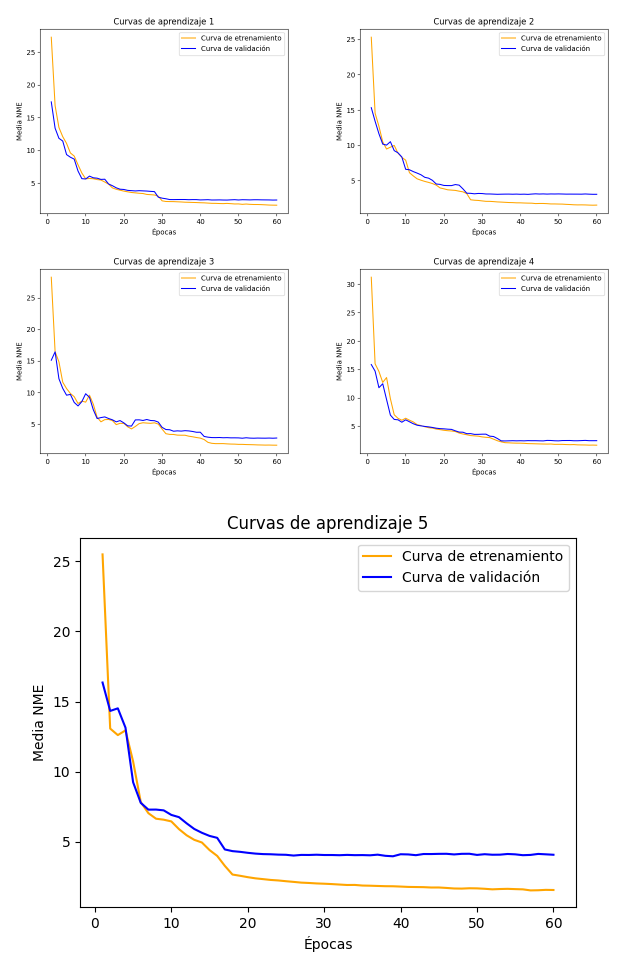
\includegraphics[width=0.9\textwidth]{img/curvas_aprendizaje_modelbase.png}
                \caption{Curvas de aprendizaje en cada partición del modelo base.}
                \label{fig:Curvas_modelbase}
            \end{figure}

            \noindent En resumen, los resultados parecen buenos para tratarse de una primera aproximación. Sin embargo, consideramos que debido a la gran variabilidad del dataset tanto en posturas, como en calidad e iluminación de imagen, la reconstrucción de las imágenes se ha resentido, especialmente en las imágenes de perfil. Esto provoca que el modelo también marque peor los landmarks, por lo que vamos a intentar mejorar esto en los próximos modelos.

        \subsubsection{Modelo con reentrenamiento del encoder}
            \noindent A la luz de los resultados anteriores, vamos a cambiar el modelo de manera que ahora junto con las ITLs (que seguirán usando el mismo optimizador con los mismos parámetros por defecto), vamos a entrenar los pesos del \textit{encoder}. Con este enfoque queremos enseñar a la red a codificar mejor la información presente en las imágenes del dataset (que son más difíciles que las de los datasets empleados anteriormente), a la par que la enseñamos a marcar landmarks en las mismas. 

            \medskip

            \noindent Este proceso no produce overfitting pues durante las etapas de entrenamiento los pesos del \textit{decoder} permanecerán congelados, y serán únicamente los pesos del \textit{encoder} los que se actualicen con backpropagation. El optimizador empleado para el entrenamiento del \textit{encoder} es Adam, el mismo que ellos emplean y los parámetros se mantienen por defecto ($\beta_1=0.9$ y $\beta_2=0.999$) a excepción del \textit{learning rate}, que se establece a $2^{-6}$, en vez de $2^{-5}$. El motivo por el cual se realiza este cambio es porque experimentando en esta fase se vio que con el antiguo \textit{Learning rate} no se conseguía mejorar apenas la reconstrucción en validación, pues durante el entrenamiento el error de reconstrucción pronto quedaba estancado en un valor. Para evitar esto se optó por reducir el learning rate consiguiendo mejorar un poco más el error de reconstrucción. El entrenamiento duró en total \textbf{100 épocas}, pues el modelos mejora más lentamente en el reconocimiento de landmarks.

            \begin{table}[!ht]
                \centering
                \caption{Media del error NME obtenido por landmark entre todas las particiones de cross-validation.}
                \begin{tabular}{|l|l|l|}
                \hline
                    ~ & Landmark & Media NME por landmark \\ \hline
                    0 & Menton & 3.997 \\ \hline
                    1 & Gnathion & 2.606 \\ \hline
                    2 & Pogonion & 2.546 \\ \hline
                    3 & Prosthion & 1.048 \\ \hline
                    4 & Labiale Superius & 2.04 \\ \hline
                    5 & Subnasale & 1.992 \\ \hline
                    6 & Nasion & 2.099 \\ \hline
                    7 & Glabella & 2.736 \\ \hline
                    8 & Vertex & 5.89 \\ \hline
                    9 & Left Gonion & 5.789 \\ \hline
                    10 & Right Gonion & 5.301 \\ \hline
                    11 & Left Zygion & 5.288 \\ \hline
                    12 & Right Zygion & 6.291 \\ \hline
                    13 & Left Alare & 1.959 \\ \hline
                    14 & Right Alare & 2.232 \\ \hline
                    15 & Left Endocanthion & 1.71 \\ \hline
                    16 & Right Endocanthion & 1.647 \\ \hline
                    17 & Left Exocanthion & 1.733 \\ \hline
                    18 & Right Exocanthion & 1.746 \\ \hline
                    19 & Left Tragion & 3.633 \\ \hline
                    20 & Right Tragion & 5.252 \\ \hline
                    21 & Labiale inferius & 1.688 \\ \hline
                    22 & Trichion & 4.762 \\ \hline
                    23 & Supramentale & 1.991 \\ \hline
                    24 & Left Frontotemporale & 2.452 \\ \hline
                    25 & Right Frontotemporale & 3.282 \\ \hline
                    26 & Left Frontozygomaticus & 1.499 \\ \hline
                    27 & Right Frontozygomaticus & 2.516 \\ \hline
                    28 & Left Midsurpaorbital & 1.178 \\ \hline
                    29 & Right Midsupraorbital & 1.348 \\ \hline
                \end{tabular}
                \label{table:Encode_landmarkresume}
            \end{table}
        
        \noindent Como podemos observar en la \autoref{table:Encode_landmarkresume}, los valores son muy similares a los del modelo base, pese a que este ha entrenado durante más épocas. El \textit{Prosthion} sigue siendo el landmark mejor marcado con un valor del error NME ligeramente superior al del modelo base, sin embargo la verdadera mejora se aprecia en el marcado de landmarks de los perfiles, al mejorar la reconstrucción de los mismos, el \textit{Right Gonion} ha bajado su error considerablemente con respecto al modelbase.
        
        \medskip
        
        \noindent Por otro lado, como podemos ver en las tablas de validación por imágenes en el \autoref{ap:apendiceB}, el error de reconstrucción ha mejorado muy ligeramente en las imágenes de validación, y no supone una mejora considerable con respecto al modelo base. 

        \medskip

        \noindent Finalmente podemos observar en las curvas de aprendizaje para este modelo en la \autoref{fig:curvas_encoder} que comienza a bajar la capacidad de generalización del modelo a partir de la época 20 aproximadamente. El error de entrenamiento comienza a descender muy lentamente mientras que el de validación se mantiene constante.

        \begin{figure}[!h]
            \centering
            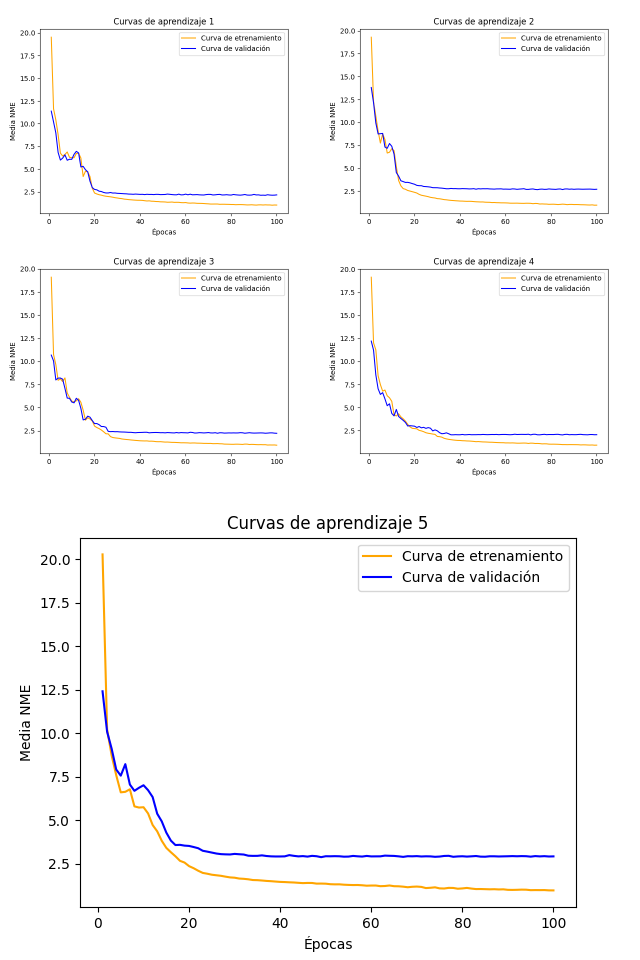
\includegraphics[width=0.9\textwidth]{img/curvas_encoder.png}
            \caption{Curvas de aprendizaje en cada partición del modelo de finetuning del encoder.}
            \label{fig:curvas_encoder}
        \end{figure}

        \medskip

        \noindent Viendo estos resultados no parece muy prometedora esta línea de investigación, por lo que vamos a cambiar el enfoque sobre el finetuning en el siguiente modelo.

        \subsubsection{Modelo con reentrenamiento del decoder}
            \noindent Del mismo modo en que se experimentó con el \textit{encoder} se hizo con el \textit{decoder}. En este enfoque asumimos que el framework sabe codificar correctamente las imágenes pero que no realiza lo suficientemente bien la reconstrucción de las mismas debido a la alta variabilidad del dataset. Esta etapa es completamente análoga a la del modelo anterior (incluyendo el mismo tipo de optimizadores, parámetros y regiones que permanecen congeladas de la red), pero actualizando los pesos del \textit{decoder}.

            \begin{table}[!ht]
                \centering
                \caption{Media del error NME obtenido por landmark en validación empleando todas las particiones de cross-validation.}
                \begin{tabular}{|l|l|l|}
                \hline
                    ~ & Landmark & Media NME por landmark \\ \hline
                    0 & Menton & 3.991 \\ \hline
                    1 & Gnathion & 2.634 \\ \hline
                    2 & Pogonion & 2.585 \\ \hline
                    3 & Prosthion & 0.97 \\ \hline
                    4 & Labiale Superius & 2.059 \\ \hline
                    5 & Subnasale & 2.089 \\ \hline
                    6 & Nasion & 2.275 \\ \hline
                    7 & Glabella & 2.912 \\ \hline
                    8 & Vertex & 6.137 \\ \hline
                    9 & Left Gonion & 5.665 \\ \hline
                    10 & Right Gonion & 5.468 \\ \hline
                    11 & Left Zygion & 5.29 \\ \hline
                    12 & Right Zygion & 6.14 \\ \hline
                    13 & Left Alare & 2.051 \\ \hline
                    14 & Right Alare & 2.295 \\ \hline
                    15 & Left Endocanthion & 1.827 \\ \hline
                    16 & Right Endocanthion & 1.61 \\ \hline
                    17 & Left Exocanthion & 1.809 \\ \hline
                    18 & Right Exocanthion & 1.734 \\ \hline
                    19 & Left Tragion & 4.163 \\ \hline
                    20 & Right Tragion & 4.791 \\ \hline
                    21 & Labiale inferius & 1.627 \\ \hline
                    22 & Trichion & 5.196 \\ \hline
                    23 & Supramentale & 1.839 \\ \hline
                    24 & Left Frontotemporale & 2.474 \\ \hline
                    25 & Right Frontotemporale & 3.009 \\ \hline
                    26 & Left Frontozygomaticus & 1.525 \\ \hline
                    27 & Right Frontozygomaticus & 2.395 \\ \hline
                    28 & Left Midsurpaorbital & 1.191 \\ \hline
                    29 & Right Midsupraorbital & 1.48 \\ \hline
                \end{tabular}
                \label{table:Decoder_landmarksresume}
            \end{table}          
            
            \medskip 

            \noindent De nuevo los errores por landmark que se muestran en la tabla \autoref{table:Decoder_landmarksresume} es muy similar a la de los dos modelos anteriores, por lo que no hemos logrado una gran mejora con este modelo tampoco. Lo único digno de mención es que de nuevo los landmarks que son más visibles en imágenes de perfil han reducido su error debido a la leve mejora de la reconstrucción de las imágenes. 

            \medskip

            \noindent Por otro lado, en lo que respecta a los errores promedio de todos los landmarks por imagen, las tablas por partición se pueden consultar en \autoref{ap:apendiceC}, aunque los resultados son muy similares a los de los modelos anteriores. El error de reconstrucción de nuevo no mejora apenas y los errores NMEs promedio son muy parecidos a los de los otros modelos. 

            \medskip

            \noindent Las curvas de aprendizaje se pueden ver en la \autoref{fig:curvas_decoder}, y vuelven a mostrar un ligero overfitting a partir de la época $30$-$40$, en la mayoría de casos. 
            
            \begin{figure}[!h]
                \centering
                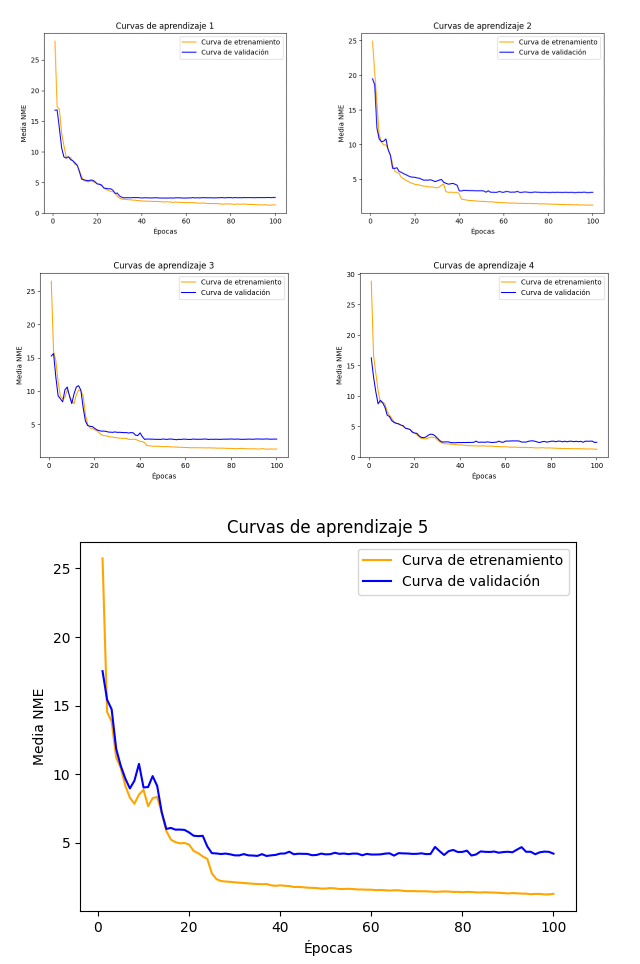
\includegraphics[width=0.9\textwidth]{img/curvas_decoder.png}
                \caption{Curvas de aprendizaje en cada partición del modelo de finetuning del encoder.}
                \label{fig:curvas_decoder}
            \end{figure}

            \medskip

            \noindent Tras los resultados obtenidos se ha optado por abandonar también esta línea de investigación pues se obtienen resultados muy similares al modelo base y se debe entrenar por mucho más tiempo ($100$ épocas frente a $40$ del modelo base). 

        \subsubsection{Modelo con Data Augmentation}
            \noindent Comparando los tres resultados anteriores, el modelo base sigue siendo el más prometedor, por lo que en lugar de mejorar el error de reconstrucción vamos a centrarnos en mejorar el marcado de landmarks. Como pudimos ver en el modelo base, se consiguieron buenos resultados del \textit{NME} pese a haber entrenado sin realizar técnicas de \textit{data augmentation}. Es por ello que en este segundo experimento vamos a realizar los siguientes cambios en el entrenamiento: 
            
            \begin{itemize}
                \item En primer lugar se realizará un entrenamiento del modelo similar al del modelo base durante $40$ épocas.
                \item Tras esto, se entrenará el modelo con el dataset al cual se le aplicarán técnicas de data augmentation, para aumentar el número de datos de entrenamiento e incrementar aún más la variabilidad de los mismos, de manera que cada imagen del dataset sufrirá de manera aleatoria una traslación ($\pm 4\%$), un reescalado ($\pm 5\%$), una rotación ($\pm 30$ grados) y oclusiones parciales. El entrenamiento en este nuevo dataset será durante $40$ épocas tras acabar las de la etapa anterior. 
                %TODO PONER IMÁGENES DE EJEMPLO DE LAS TRANSFORMACIONES
                \item En total serán \textbf{$80$ épocas} de entrenamiento sumando las dos etapas anteriores.
            \end{itemize}

            \medskip

            \noindent De nuevo, el resto de parámetros continuarán con los valores por defecto de la etapa anterior, pues los resultados obtenidos han sido buenos hasta el momento y nada sugiere tener que cambiarlos.

            \begin{table}[!ht]
                \centering
                \caption{Media del error NME obtenido por landmark en validación empleando todas las particiones de cross-validation con el modelo de data augmentation.}
                \begin{tabular}{|l|l|l|}
                \hline
                    ~ & Landmark & Media NME por landmark \\ \hline
                    0 & Menton & 3.006 \\ \hline
                    1 & Gnathion & 1.497 \\ \hline
                    2 & Pogonion & 1.359 \\ \hline
                    3 & Prosthion & 0.815 \\ \hline
                    4 & Labiale Superius & 1.531 \\ \hline
                    5 & Subnasale & 1.272 \\ \hline
                    6 & Nasion & 1.241 \\ \hline
                    7 & Glabella & 1.545 \\ \hline
                    8 & Vertex & 3.99 \\ \hline
                    9 & Left Gonion & 1.846 \\ \hline
                    10 & Right Gonion & 1.673 \\ \hline
                    11 & Left Zygion & 3.322 \\ \hline
                    12 & Right Zygion & 4.441 \\ \hline
                    13 & Left Alare & 1.585 \\ \hline
                    14 & Right Alare & 1.362 \\ \hline
                    15 & Left Endocanthion & 1.227 \\ \hline
                    16 & Right Endocanthion & 1.129 \\ \hline
                    17 & Left Exocanthion & 1.186 \\ \hline
                    18 & Right Exocanthion & 1.12 \\ \hline
                    19 & Left Tragion & 2.066 \\ \hline
                    20 & Right Tragion & 2.234 \\ \hline
                    21 & Labiale inferius & 1.032 \\ \hline
                    22 & Trichion & 3.37 \\ \hline
                    23 & Supramentale & 1.109 \\ \hline
                    24 & Left Frontotemporale & 1.386 \\ \hline
                    25 & Right Frontotemporale & 1.826 \\ \hline
                    26 & Left Frontozygomaticus & 1.036 \\ \hline
                    27 & Right Frontozygomaticus & 1.057 \\ \hline
                    28 & Left Midsurpaorbital & 0.854 \\ \hline
                    29 & Right Midsupraorbital & 0.945 \\ \hline
                \end{tabular}
                \label{table:Daugmentation_landmarksresume}
            \end{table}

            \medskip

            \noindent Como podemos ver en la \autoref{table:Daugmentation_landmarksresume}, los errores se han reducido en general en todos los landmarks, además la red ha conseguido aprender a marcar con un alto grado de precisión los puntos que se ven en el perfil de la cara. El punto mejor marcado sería el \textit{prosthion} de nuevo, y el peor marcado el \textit{right zygion}. Sin embargo, la diferencia en términos de error entre ambos es mucho menor que en el caso del modelo base. 

            \medskip

            \noindent 
        \subsubsection{Modelo \textit{fine-tuning}}
    \subsection{Comparación de resultados}
\endinput
%------------------------------------------------------------------------------------
% FIN DEL CAPÍTULO. 
%------------------------------------------------------------------------------------



